
%%%%%%%%%%%%%%%%%%%%%%%%%%%%%%%%%%%%%%%%%%%%%%%%
%%%%%%%%%%%%%%%%%%%%%%%%%%%%%%%%%%%%%%%%%%%%%%%%
\begin{frame}
  \frametitle{Scientific software devel. at MDLS using Kokkos}

{\small
  \begin{minipage}{0.69\linewidth}
    \begin{itemize}
    % \item \myhref{https://github.com/pkestene/ramsesGPU}{RamsesGPU} (2009-2014, CUDA) : CFD on full cartesian grid, finite volumes, magnetorotationnal instability study,
    %   \begin{itemize}
    %   \item run on Curie (2013-14, 256 GPUs, Nvidia M2090), with {\bf S. Fromang} (DRF/IRFU/DAp)
    %   \item run on \myhref{https://bluewaters.ncsa.illinois.edu/}{NCSA blueWaters} (2014-15, 1024 GPUs, Nvidia K20)
    %   \end{itemize}
    \item {\bf since 2016:} R\&D using \myhref{https://github.com/kokkos/kokkos}{MPI+Kokkos}\\
      mini-app \myhref{https://github.com/pkestene/euler_kokkos}{EulerKokkos} $\Rightarrow$ \myhref{https://www.gitlab.erc-atmo.eu/erc-atmo/ark}{ARK} (\textcolor{darkgreen}{\bf high/low Mach flow with well-balanced gravity}) by \underline{\bf T. Padioleau}, {\bf P. Tremblin} (DRF/MDLS), {\bf S. Kokh} (DES/STMF), \myhref{https://www.gitlab.erc-atmo.eu/erc-atmo/ARK-RT}{ARK-RT} (Radiative transfert)
   \item<1-> {\bf 2018:} \myhref{https://gitlab.maisondelasimulation.fr/pkestene/LBM_saclay/}{LBM\_Saclay} with {\bf A. Cartalade} and {\bf A. Genty} (DES/STMF)\\
      %Master2: \underline{W. Verdier} : film boiling\\
      PhD: \underline{\bf W. Verdier, T. Boutin} : Two-phase flow (Navier-Stokes + phase fields models) with phase change using \textcolor{darkgreen}{\bf Lattice Boltzmann methods} for studying demixing process in glasses, dissolution in porous media.
    \item<1-> {\bf 2017-2018:} \myhref{https://github.com/pkestene/ppkMHD}{ppkMHD} MPI+Kokkos implementation of high order \textcolor{darkgreen}{\bf spectral difference method} (SDM)\\
       \begin{center}
        \includegraphics<1->[width=0.42\linewidth]{images/ppkMHD/jet_mach27_sdm_deg3_deg4_t0p6}
        \includegraphics<1->[width=0.42\linewidth]{images/lbm_saclay/lbm_saclay_film_boiling2}\\
        \only<1->{\tiny (left) ppkMHD (MPI+Kokkos: high Mach (M=27) jet}\\
        \only<1->{\tiny (right) LBM\_Saclay (MPI+Kokkos): film boiling (2019, Verdier, STMF)}
      \end{center}
    %\item<1-> {\bf 2018:} \myhref{https://www.parco.org/ParCo2019/index.html}{PTC Kokkos NDT} (Non-destructive Testing) with {\bf V. Bergeaud} (DRT/DISC) and \underline{A. Audi}: portability of selected CIVA algorithms
    \end{itemize}
  \end{minipage}
  %
  \begin{minipage}[t][\textheight]{0.3\linewidth}
    \begin{center}
      %\includegraphics<1-2>[width=0.85\linewidth]{images/ramsesgpu/ramsesgpu_mri_by}
      %\only<1-2>{\scriptsize MRI: $800\times 1600 \times 800$}
      %\only<1-2>{\vspace{3cm}}

      \includegraphics<-1>[width=0.70\linewidth]{images/ark/ark_rayleigh_benard}

      \only<-1>{\tiny ARK Rayleigh-Benard instability (2019, Padioleau, MDLS)}

      \includegraphics<1->[width=0.70\linewidth]{images/ark/ark_weak_scaling_jean_zay}

      \only<1->{\tiny ARK GPU weak-scaling, $4960^3$ (2019, Daley-Yates, MDLS, Jean Zay/IDRIS)}

      %\includegraphics<1->[width=0.70\linewidth]{images/lbm_saclay/lbm_saclay_film_boiling2}

      %\only<1->{\tiny LBM\_Saclay (MPI+Kokkos): film boiling (2019, Verdier, STMF)}

      %\includegraphics<1->[width=0.4\linewidth]{images/ndt/tfm/tfm_step1}

      \vfill

    \end{center}
  \end{minipage}
}

\end{frame}

%%%%%%%%%%%%%%%%%%%%%%%%%%%%%%%%%%%%%%%%%%%%%%%%
%%%%%%%%%%%%%%%%%%%%%%%%%%%%%%%%%%%%%%%%%%%%%%%%
%%%%%%%%%%%%%%%%%%%%%%%%%%%%%%%%%%%%%%%%%%%%%%%%
\begin{frame}[fragile=singleslide]
  \frametitle{Prototyping adaptive mesh refinement with Kokkos}

  \begin{minipage}{0.52\linewidth}
     \begin{itemize}
     \item At CEA/DRF/IRFU ({\bf \underline{A. Durocher, M. Delorme}}) :\\
        \textcolor{darkgreen}{\bf Dyablo $=$ A C++ software platform for octree-based AMR CFD applications} using external libraries:
    \begin{itemize}
    \item (\myhref{https://optimad.github.io/bitpit/}{PABLO}) for distributed mesh management and AMR algorithms
    \item \myhref{https://github.com/kokkos/kokkos}{Kokkos} for shared mem. parallelism (CPU/GPU)
    \end{itemize}
  \item Mini-app focused on single-node AMR running entirely on device (GPU) written in Kokkos for LBM applications
     \begin{itemize}
     %\item \textcolor{blue}{\bf P. Kestener} (0.5 FTE, in 2019): original design, core framework, finite volume scheme implementation Kokkos/OpenMP, hashmap refactoring
     %\item \textcolor{blue}{\bf A. Durocher} (DRF/IRFU/DEDIP, 1.0 FTE since 09/2020): core framework, continuous integration, Kokkos/CUDA adaptation, collaboration with DRF/IRFU/DAp (F. Bournaud, P. Hennebelle), P. Tremblin (DRF/MDLS)
     %\item \textcolor{blue}{\bf M. Delorme} (DRF/IRU/DAp, 0.5 FTE, since Jan. 2020): physics modules (ERC WholeSun, PI: S. Brun)
     \item \underline{\bf E. Stavropoulos Vasilakis} (CEA/DES/STMF), started {\bf 02/2021}, Lattice Boltzmann numerical scheme implementation
     \end{itemize}
  \end{itemize}
  \end{minipage}
  %
  \begin{minipage}{0.47\linewidth}
    \begin{center}
      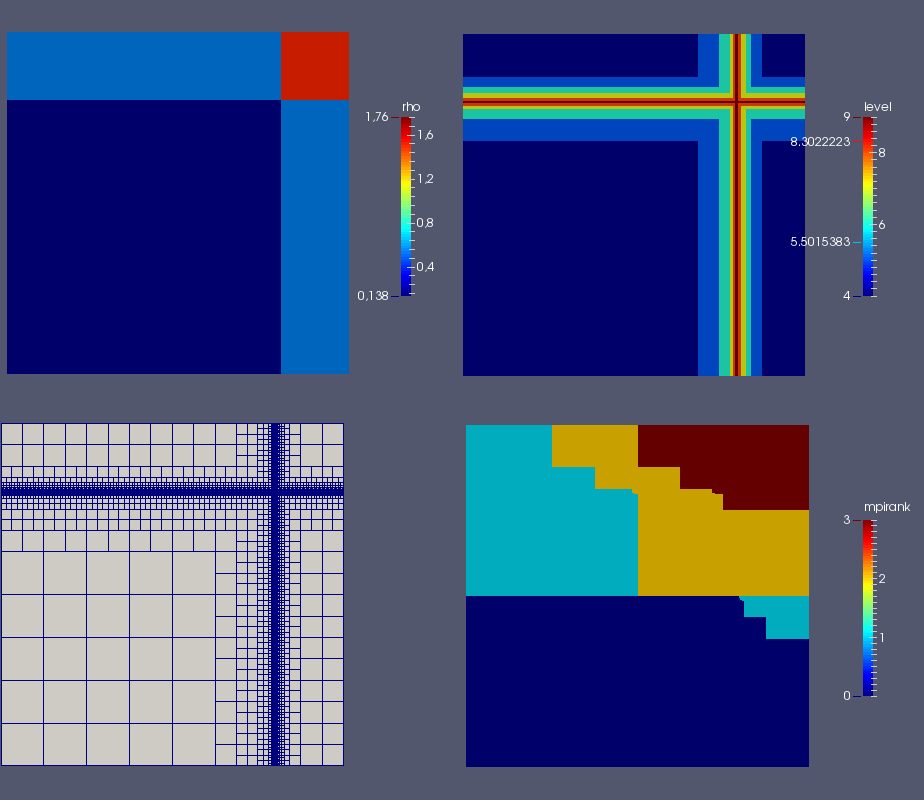
\includegraphics[height=3.0cm]{./images/canop/piecewise_const_prob3/piecewise_const_prob3_t0p0}\vspace{0.3cm}

      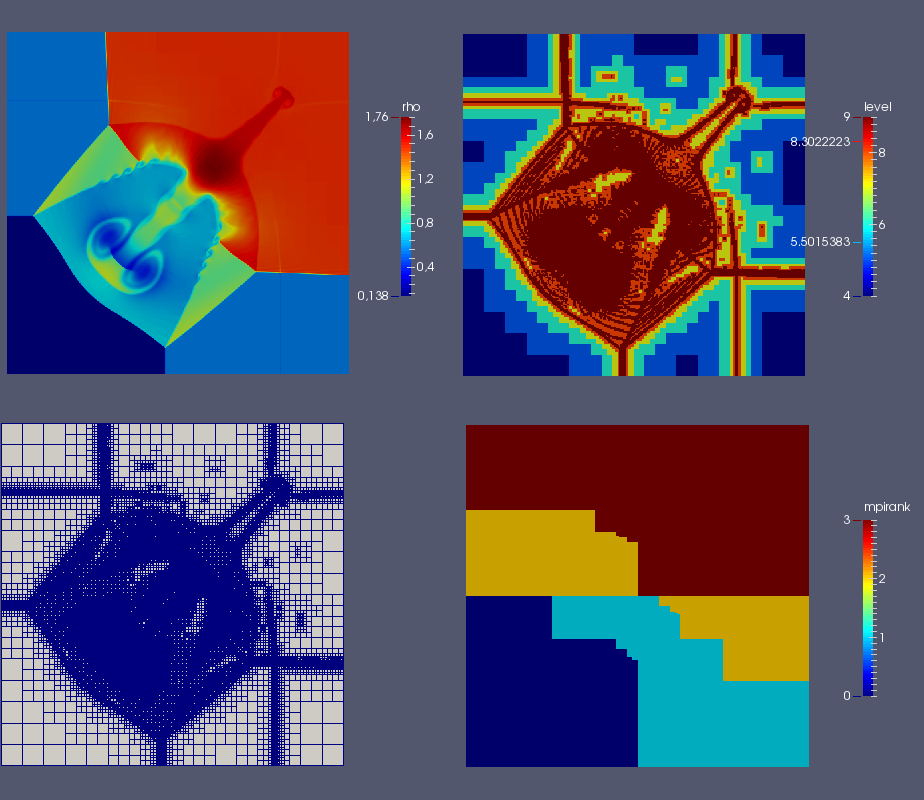
\includegraphics[height=3.0cm]{./images/canop/piecewise_const_prob3/piecewise_const_prob3_t0p8}\\
      {\bf code CanoP (\myhref{https://www.p4est.org/}{p4est})}
    \end{center}
  \end{minipage}
\end{frame}

%%%%%%%%%%%%%%%%%%%%%%%%%%%%%%%%%%%%%%%%%%%%%%%%
%%%%%%%%%%%%%%%%%%%%%%%%%%%%%%%%%%%%%%%%%%%%%%%%
\begin{frame}[fragile=singleslide]
  \frametitle{Kokkos + AMR = khamr}

  \begin{itemize}
  \item {\bf Sand box / testing ideas of generic multi-architecture AMR} %\myhref{https://gitlab.maisondelasimulation.fr/pkestene/khamr}{khamr}
  \item testing sorting algorithmes with Kokkos, bucket sort, ...
  \item testing Morton index and data containers (encode/decode, use level/tree id)
    {\scriptsize
      \begin{minted}[autogobble=true]{c++}
        KOKKOS_INLINE_FUNCTION
        uint64_t morton_key(const int ix, const int iy, const int iz)
        {
          uint64_t key = 0;
          key |= splitBy3<3>(ix) | splitBy3<3>(iy) << 1 | splitBy3<3>(iz) << 2;
          return key;
        } // morton_key - 3d
      \end{minted}
    }
  \item testing parallel hash tables
    \begin{center}
      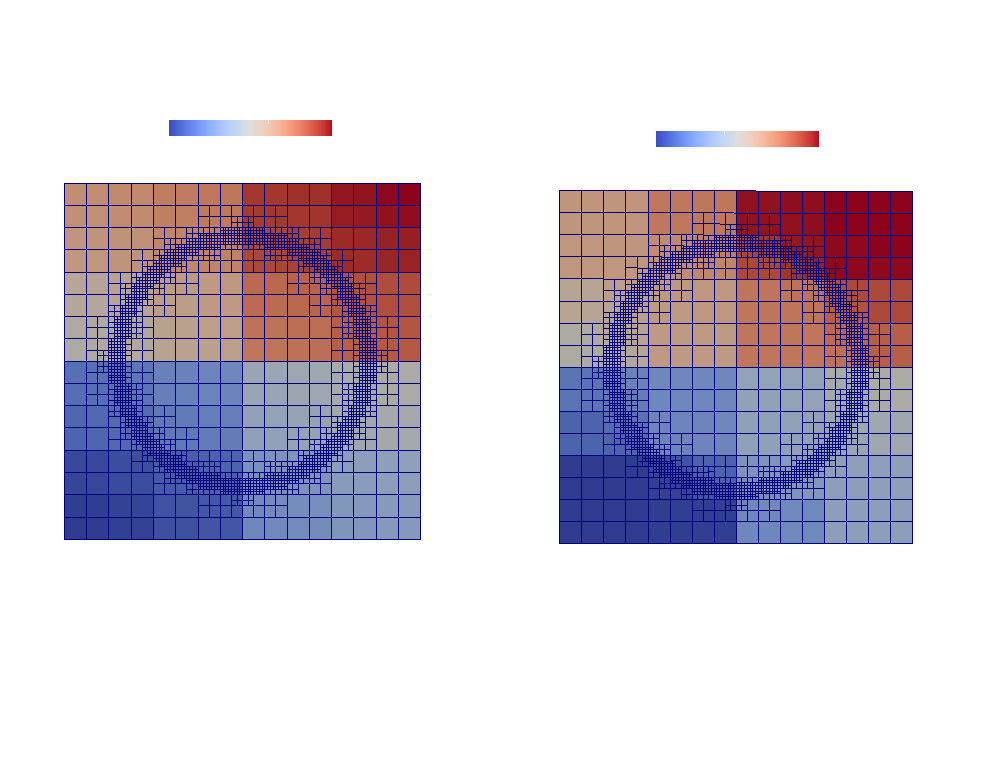
\includegraphics[width=5cm]{images/khamr/khamr}
    \end{center}
  \end{itemize}

\end{frame}
